\documentclass[tikz,crop,convert={density=200,outext=.png},border=0.4cm]{standalone}

\usepackage{pgfplots}
\usepackage{amsmath}
\usetikzlibrary{arrows.meta}
\usepackage{physics}
\usepackage{xcolor}
\definecolor{mixed_1}{RGB}{8,48,107}
\pgfplotsset{compat=newest,
    %width=6cm,
    %height=3cm,
    scale only axis=true,
    max space between ticks=25pt,
    try min ticks=5,
    every axis/.style={
        axis y line=middle,
        axis x line=middle,
        axis line style={thick,->,>=latex, shorten >=-.3cm}
    },
    every axis plot/.append style={thick},
    tick style={black, thick},
}
\tikzset{
    semithick/.style={line width=0.8pt},
}
\usepgfplotslibrary{groupplots}
\usepgfplotslibrary{dateplot}
% Document begins
\begin{document}
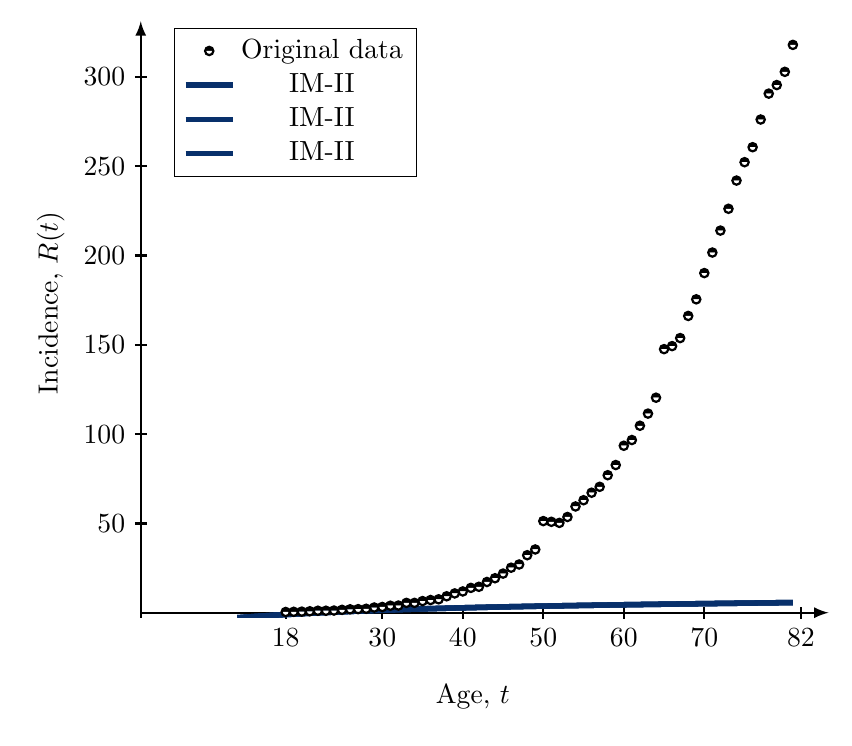
\begin{tikzpicture}
  % The axis of the plot
\begin{axis}[
    %title={Model: $\dv{y}{t}=\frac{2y}{t}$ with solution $y(t)=C_1t^2$\\Symmetry: $\Gamma_{\epsilon}=(t,y)\mapsto\left(\exp\left(\epsilon\right)t,\exp\left(-\epsilon\right)y\right)$},
    title style = {align=left},
    xlabel={Age, $t$},
    ylabel={Incidence, $R(t)$},
    %ylabel={Logarithm of Incidence, $\ln\left(R(t)\right)$},    
    % ylabel={Incidence, $R(t)$},
    x label style={at={(axis description cs:0.5,-0.1)},anchor=north},
    y label style={at={(axis description cs:-0.1,0.55)},rotate=90,anchor=south},    
    % xmin=-27, xmax=5,
    xmin=0, xmax=82.5,
    xtick={0,18,30,40,...,60,70,82},    
    %ymin=-20, ymax=20,
    %xtick={-30,-27,...,9},
    %ytick={-15,-10,...,15},
    legend style={at={(axis description cs:0.05,0.9)},anchor=west},    
    %legend pos=north west,
    %ymajorgrids=true,
    grid style=dashed,
]
% Plot the data
\addplot[
only marks, mark=halfcircle*,mark size=1.5pt,color=black,
]
coordinates {%
(18.0,0.4)
(19.0,0.5)
(20.0,0.6)
(21.0,0.8)
(22.0,1.1)
(23.0,1.1)
(24.0,1.2)
(25.0,1.6)
(26.0,1.9)
(27.0,2.0)
(28.0,2.2)
(29.0,2.9)
(30.0,3.2)
(31.0,3.8999999999999995)
(32.0,4.0)
(33.0,5.5)
(34.0,5.5)
(35.0,6.499999999999999)
(36.0,7.1000000000000005)
(37.0,7.499999999999999)
(38.0,9.2)
(39.0,10.8)
(40.0,11.9)
(41.0,13.9)
(42.0,14.5)
(43.0,17.2)
(44.0,19.299999999999997)
(45.0,21.9)
(46.0,25.199999999999996)
(47.0,27.0)
(48.0,32.2)
(49.0,35.4)
(50.0,51.300000000000004)
(51.0,50.9)
(52.0,50.29999999999999)
(53.0,53.60000000000001)
(54.0,59.50000000000001)
(55.0,62.99999999999999)
(56.0,67.19999999999999)
(57.0,70.5)
(58.0,77.00000000000001)
(59.0,82.69999999999997)
(60.0,93.50000000000001)
(61.0,96.69999999999996)
(62.0,104.69999999999999)
(63.0,111.5)
(64.0,120.39999999999995)
(65.0,147.59999999999997)
(66.0,149.29999999999995)
(67.0,153.80000000000004)
(68.0,166.20000000000005)
(69.0,175.50000000000009)
(70.0,190.2)
(71.0,201.70000000000007)
(72.0,213.99999999999994)
(73.0,226.20000000000007)
(74.0,242.00000000000009)
(75.0,252.3000000000001)
(76.0,260.70000000000005)
(77.0,276.20000000000005)
(78.0,290.7000000000001)
(79.0,295.50000000000006)
(80.0,302.8999999999999)
(81.0,318.0)
};
\addlegendentry{Original data}

% Plot the model
\addplot[
color=mixed_1,line width=2pt,
]
coordinates {%
(12.0,-2.822037098690565)
(13.0,-2.490595180964096)
(14.0,-2.1733550910308974)
(15.0,-1.8696886611176815)
(16.0,-1.5789918138264785)
(17.0,-1.300683330905735)
(18.0,-1.034203723154178)
(19.0,-0.779014205171733)
(20.0,-0.5345957762981026)
(21.0,-0.3004484064514763)
(22.0,-0.07609032289094486)
(23.0,0.13894260863046792)
(24.0,0.3450974171055936)
(25.0,0.5428044844934252)
(26.0,0.7324779407701145)
(27.0,0.9145160083349522)
(28.0,1.0893013083831682)
(29.0,1.2572011414023234)
(30.0,1.4185677530292717)
(31.0,1.5737385952205258)
(32.0,1.7230365911517747)
(33.0,1.8667704105845906)
(34.0,2.005234760724201)
(35.0,2.138710695931278)
(36.0,2.2674659481146073)
(37.0,2.391755278271762)
(38.0,2.511820848493753)
(39.0,2.627892612821657)
(40.0,2.7401887246382133)
(41.0,2.848915957783549)
(42.0,2.9542701382815877)
(43.0,3.0564365834271126)
(44.0,3.1555905449852526)
(45.0,3.251897653367334)
(46.0,3.3455143598428143)
(47.0,3.436588374102024)
(48.0,3.525259094777378)
(49.0,3.6116580308434885)
(50.0,3.695909212134694)
(51.0,3.778129587530426)
(52.0,3.858429409656028)
(53.0,3.9369126052232595)
(54.0,4.013677130386733)
(55.0,4.088815310718076)
(56.0,4.162414165597813)
(57.0,4.23455571699625)
(58.0,4.305317282760147)
(59.0,4.374771754643267)
(60.0,4.442987861418055)
(61.0,4.510030417484813)
(62.0,4.575960557456043)
(63.0,4.640835957239325)
(64.0,4.704711042174288)
(65.0,4.767637182799829)
(66.0,4.829662878838605)
(67.0,4.89083393198855)
(68.0,4.951193608107267)
(69.0,5.01078278936584)
(70.0,5.069640116935026)
(71.0,5.127802124749971)
(72.0,5.185303364880268)
(73.0,5.242176525011078)
(74.0,5.298452538518819)
(75.0,5.354160687601952)
(76.0,5.409328699904155)
(77.0,5.463982839043979)
(78.0,5.518147989442147)
(79.0,5.571847735815223)
(80.0,5.625104437682597)
(81.0,5.677939299212673)
};
\addlegendentry{IM-II}
\addplot[
color=mixed_1,line width=2pt,
]
coordinates {%
(12.0,-2.822037098690565)
(13.0,-2.490595180964096)
(14.0,-2.1733550910308974)
(15.0,-1.8696886611176815)
(16.0,-1.5789918138264785)
(17.0,-1.300683330905735)
(18.0,-1.034203723154178)
(19.0,-0.779014205171733)
(20.0,-0.5345957762981026)
(21.0,-0.3004484064514763)
(22.0,-0.07609032289094486)
(23.0,0.13894260863046792)
(24.0,0.3450974171055936)
(25.0,0.5428044844934252)
(26.0,0.7324779407701145)
(27.0,0.9145160083349522)
(28.0,1.0893013083831682)
(29.0,1.2572011414023234)
(30.0,1.4185677530292717)
(31.0,1.5737385952205258)
(32.0,1.7230365911517747)
(33.0,1.8667704105845906)
(34.0,2.005234760724201)
(35.0,2.138710695931278)
(36.0,2.2674659481146073)
(37.0,2.391755278271762)
(38.0,2.511820848493753)
(39.0,2.627892612821657)
(40.0,2.7401887246382133)
(41.0,2.848915957783549)
(42.0,2.9542701382815877)
(43.0,3.0564365834271126)
(44.0,3.1555905449852526)
(45.0,3.251897653367334)
(46.0,3.3455143598428143)
(47.0,3.436588374102024)
(48.0,3.525259094777378)
(49.0,3.6116580308434885)
(50.0,3.695909212134694)
(51.0,3.778129587530426)
(52.0,3.858429409656028)
(53.0,3.9369126052232595)
(54.0,4.013677130386733)
(55.0,4.088815310718076)
(56.0,4.162414165597813)
(57.0,4.23455571699625)
(58.0,4.305317282760147)
(59.0,4.374771754643267)
(60.0,4.442987861418055)
(61.0,4.510030417484813)
(62.0,4.575960557456043)
(63.0,4.640835957239325)
(64.0,4.704711042174288)
(65.0,4.767637182799829)
(66.0,4.829662878838605)
(67.0,4.89083393198855)
(68.0,4.951193608107267)
(69.0,5.01078278936584)
(70.0,5.069640116935026)
(71.0,5.127802124749971)
(72.0,5.185303364880268)
(73.0,5.242176525011078)
(74.0,5.298452538518819)
(75.0,5.354160687601952)
(76.0,5.409328699904155)
(77.0,5.463982839043979)
(78.0,5.518147989442147)
(79.0,5.571847735815223)
(80.0,5.625104437682597)
(81.0,5.677939299212673)
};
\addlegendentry{IM-II}
\addplot[
color=mixed_1,line width=2pt,
]
coordinates {%
(12.0,-2.822037098690565)
(13.0,-2.490595180964096)
(14.0,-2.1733550910308974)
(15.0,-1.8696886611176815)
(16.0,-1.5789918138264785)
(17.0,-1.300683330905735)
(18.0,-1.034203723154178)
(19.0,-0.779014205171733)
(20.0,-0.5345957762981026)
(21.0,-0.3004484064514763)
(22.0,-0.07609032289094486)
(23.0,0.13894260863046792)
(24.0,0.3450974171055936)
(25.0,0.5428044844934252)
(26.0,0.7324779407701145)
(27.0,0.9145160083349522)
(28.0,1.0893013083831682)
(29.0,1.2572011414023234)
(30.0,1.4185677530292717)
(31.0,1.5737385952205258)
(32.0,1.7230365911517747)
(33.0,1.8667704105845906)
(34.0,2.005234760724201)
(35.0,2.138710695931278)
(36.0,2.2674659481146073)
(37.0,2.391755278271762)
(38.0,2.511820848493753)
(39.0,2.627892612821657)
(40.0,2.7401887246382133)
(41.0,2.848915957783549)
(42.0,2.9542701382815877)
(43.0,3.0564365834271126)
(44.0,3.1555905449852526)
(45.0,3.251897653367334)
(46.0,3.3455143598428143)
(47.0,3.436588374102024)
(48.0,3.525259094777378)
(49.0,3.6116580308434885)
(50.0,3.695909212134694)
(51.0,3.778129587530426)
(52.0,3.858429409656028)
(53.0,3.9369126052232595)
(54.0,4.013677130386733)
(55.0,4.088815310718076)
(56.0,4.162414165597813)
(57.0,4.23455571699625)
(58.0,4.305317282760147)
(59.0,4.374771754643267)
(60.0,4.442987861418055)
(61.0,4.510030417484813)
(62.0,4.575960557456043)
(63.0,4.640835957239325)
(64.0,4.704711042174288)
(65.0,4.767637182799829)
(66.0,4.829662878838605)
(67.0,4.89083393198855)
(68.0,4.951193608107267)
(69.0,5.01078278936584)
(70.0,5.069640116935026)
(71.0,5.127802124749971)
(72.0,5.185303364880268)
(73.0,5.242176525011078)
(74.0,5.298452538518819)
(75.0,5.354160687601952)
(76.0,5.409328699904155)
(77.0,5.463982839043979)
(78.0,5.518147989442147)
(79.0,5.571847735815223)
(80.0,5.625104437682597)
(81.0,5.677939299212673)
};
\addlegendentry{IM-II}

\end{axis}
\end{tikzpicture}

\end{document}
